We call \emph{contour plot} the graph representing the value of a quantity on every mainline link at all times: the mainline links as absciss and time steps as ordinates.
Fig. \ref{fig:beats_contour}. below is an example of a density contour plot for one day on a 135 links freeway, from a traffic model output.\\
\begin{figure}[h]
	\centering
	\label{fig:beats_contour}
	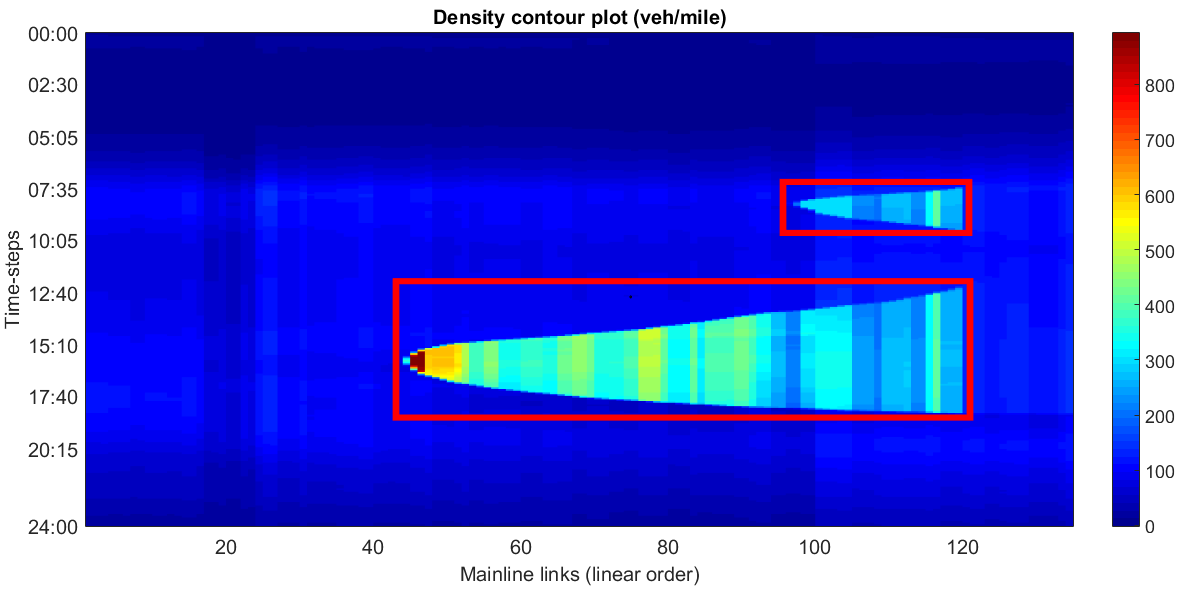
\includegraphics[width=7in]{beats_contour.png}
	\caption{Example of a density contour plot on a 135 mainline links freeway over 24h out of a traffic model output.}
\end{figure}
This plot is used to monitor easily where and when the congestion is : here, we see empirically that it is contained in the two framed parts.\\
In what follows, by analogy, we will call \emph{contour domain} the set $\mathscr{P}$=$\big\{(i,t)|\ i\in M,\ t\in\tau\big\}$ and \emph{pixel} each of its elements.\\
On the model output, we define the \emph{congested} pixels as the ones where the density exceeds some \emph{critical density} deduced for each link from the freeway and traffic models. The main feature of our calibration method is to fit the locations and times of these congested pixels to what the measurements indicate.\\
For each mainline link $i\in{M}$, we denote $d_{i}^{*}$ the critical density.
\\
We define the \emph{output congested domain} $\mathscr{C}\in\mathscr{P}$ containing the congested pixels :
\begin{equation*}
	\mathscr{C}=\big\{ (i,t)\in{\mathscr{P}}\ |\ {d_{i}(t) \geq d_{i}^{*}}\big\}
\end{equation*}
%We also define the \emph{congestion pattern} performance metric $CP$ as the signaling matrix 
%of $\mathscr{C}$ :
%\begin{equation*}
%	CP=\big(\mathds{1}_{(i,j.dt)\in \mathscr{C}}\big)_{\stackrel{i\in M}{j\in \llbracket 0,\frac{D}{dt}\rrbracket}}
%\end{equation*}
To define an error based on $\mathscr{C}$, a domain supposed to contain the congestion as to be determined.
From the data \emph{density contour plot} (partial, obtained only on the monitored links), we define a domain $\widetilde{\mathscr{C}}\subset\mathscr{P}$ fitting the congested pixels as best as it can following some criteria (how this domain is built depends on the amount of data the operator possesses and on his goals. In our case, $\widetilde{\mathscr{C}}$ was a set of rectangles containing all the congestion seen in the data contour plot).\\
%The same way we defined $CP$, we define $\widetilde(CP)$ as the signaling matrix of $\widetilde{C}$:
%\begin{equation*}
%	\widetilde{CP}=\big(\mathds{1}_{(i,j.dt)\in \mathscr{\widetilde{C}}\big)_{\stackrel{i\in M}{j\in \llbracket 0,\frac{D}{dt}\rrbracket}}
%\end{equation*}
\\
We can now define the congestion pattern error denoted $E_{CP}$ as the normalized number of wrong congestion state pixels. That is, we add one to $E_{CP}$ for each pixel that is not congested but should and for each pixel that is congested but shouldn't. We then divide this result by the number of pixels that should be congested (i.e. $Card(\widetilde{\mathscr{C}})=\sum_{t\in{\tau}}\sum_{i\in{M}}\mathds{1}_{(i,t)\in{\widetilde{\mathscr{C}}}}$).
\begin{equation*}
	E_{CP}(\vec{k})=\frac{\sum_{t\in{\tau}}\sum_{i\in{M}}\mathds{1}_{\{(i,t)\in{(\widetilde{\mathscr{C}}\backslash \mathscr{C})\cup(\mathscr{C}\backslash \widetilde{\mathscr{C}} })\}}}{\sum_{t\in{\tau}}\sum_{i\in{M}}\mathds{1}_{(i,t)\in{\widetilde{\mathscr{C}}}}}
\end{equation*}
Note that $E_{CP}$ becomes very sensible if the data does not contain much congestion (i.e. $Card(\widetilde{\mathscr{C}})<<Card(\mathscr{P})$).\\
\\
Fig. \ref{fig:cp_example}. below is a visual representation on a contour domain of $(\widetilde{\mathscr{C}}\backslash \mathscr{C})$ otherwise called \emph{false negative pixels}, $(\mathscr{C}\backslash\widetilde{\mathscr{C}})$ otherwise called \emph{false positive pixels} and $(\mathscr{C}\cap\widetilde{\mathscr{C}})\cup \big(\mathscr{P}\backslash(\mathscr{C}\cup \widetilde{\mathscr{C}})\big)$, which are the \emph{correct congestion matching} pixels. 
\\Here, $\widetilde{\mathscr{C}}$ is the yellow rectangle.
\begin{figure}[h]
	\caption{Visual example of the congestion pattern matching computation. $\widetilde{\mathscr{C}}$ is one rectangle.}
	\label{fig:cp_example}
	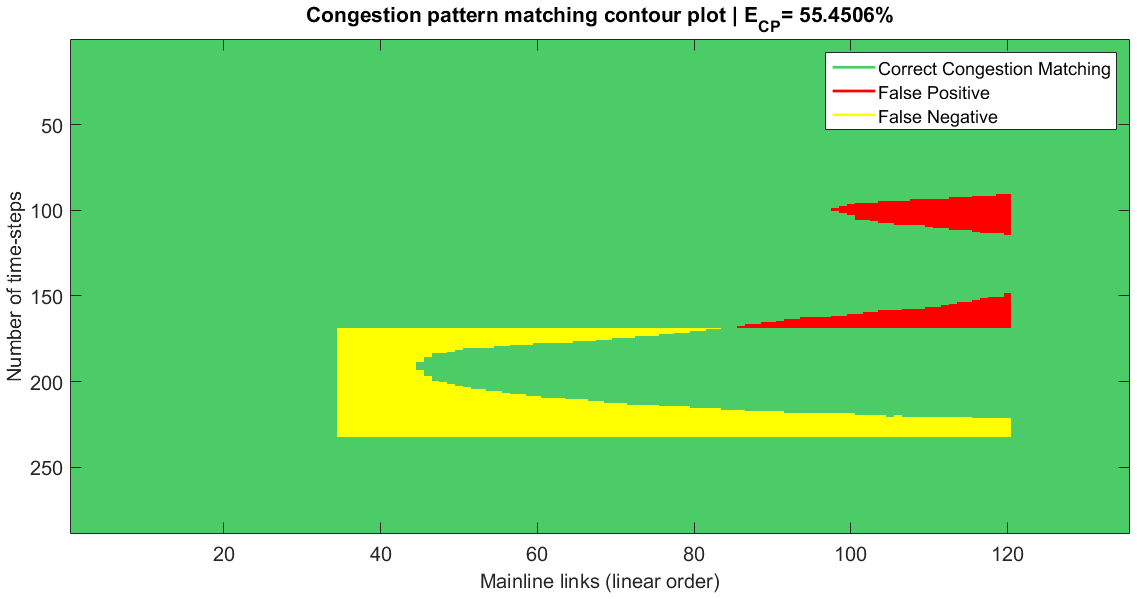
\includegraphics[width=7in]{figures/cp_example.png}
\end{figure}
